%! TEX program = xelatex

\documentclass{article}
\usepackage[a4paper, margin=3cm]{geometry}
\setlength{\parindent}{0pt}
\setlength{\parskip}{1em}
\usepackage{fontspec}
\setmainfont{Lato}

\usepackage{amsmath,amssymb,amsthm}
\usepackage{verbatim}
\usepackage{hyperref}
\usepackage{graphicx}
%\usepackage{pgfplots}
%\pgfplotsset{compat=1.16}

\title{}
\author{Mikael Myyrä}
\date{}

\begin{document}

\section*{2.-3.}

Esitetään ensin tehtävä matriisimuodossa, jotta nähdään, millainen matriisin
rakenne on ja mitä menetelmiä voidaan käyttää. Diskretoidaan
$-\Delta$ keskeisdifferenssillä
\[
  \frac{-u_{i-1,j} - u_{i+1,j} + 4u_{i,j} - u_{i,j-i} - u_{i,j+1}}{h^2}.
\]
Kaikilla reunoilla on homogeeninen Dirichlet-reunaehto, joten reunaehdot eivät
muuta yhtälöä lain\-kaan. Tehdään tuntemattoman vektorin $\mathbf{u}$
indeksointi järjestyksessä vasemmalta oikealle, ylhäältä alas. Diskreetin tehtävän
kertoimeksi tulee tällöin $M \times M$-lohkomatriisi
\[
  \frac{1}{h^2}
  \begin{bmatrix}
    T & -I \\
    -I & T & -I \\
       & \ddots & \ddots & \ddots \\
       & & -I & T & -I \\
       & & & -I & T \\
  \end{bmatrix}
\]
missä $M$ on laskentapisteiden lukumäärä y-suunnassa,
$I$ on identiteettimatriisi ja $T$ on $N \times N$-matriisi
\[
  \begin{bmatrix}
    4 & -1 \\
    -1 & 4 & -1 \\
       & \ddots & \ddots & \ddots \\
       & & -1 & 4 & -1 \\
       & & & -1 & 4 \\
  \end{bmatrix}
\]
missä puolestaan $N$ on laskentapisteiden lukumäärä x-suunnassa.

Tämä on neliömatriisi, joten LU-hajotelmaa voidaan käyttää. Tämä on myös
symmetrinen matriisi. Choleskyn hajotelma vaatii lisäksi, että se on
positiividefiniitti.  Gershgorinin ympyrälauseen
(\url{https://en.wikipedia.org/wiki/Gershgorin_circle_theorem}) perusteella
matriisi on ainakin positiivisemidefiniitti (ominaisarvot välillä $[0, 8]$),
mutta tämä ei kerro sen enempää. Laskemalla ominaisarvot matlabilla näyttää
siltä, että ne ovat aina aidosti positiivisia.  Jos tämä on totta, voidaan
käyttää Choleskyn hajotelmaa.  Tämän voisi varmasti todistaa selvittämällä
yleisen kaavan $N \times N$-kokoisen matriisin ominaisarvoille, mutta
aikaa on kulunut jo tarpeeksi sivuraiteilla, joten palaan itse tehtävään.

Matriisin rakenne vastaa myös syklisessä reduktiossa käsiteltävää matriisia.
Syklinen reduktio olisi varmaankin laskenta-ajan suhteen tehokkain tapa kääntää
tämä matriisi. Valitsen kuitenkin oppimistarkoituksessa Choleskyn hajotelman,
koska se on hieman yleiskäyttöisempi ja minulle entuudestaan vieras.
Käytän lähteenä Wikipedia-sivua \url{https://en.wikipedia.org/wiki/Cholesky_decomposition}.

Cholesky-ratkaisijan matlab-koodi:

\verbatiminput{w6_cholesky.m}

Tämän avulla tein tehtävän yhtälölle ratkaisijan, jota käytän myös seuraavassa tehtävässä:

\verbatiminput{w6_solver.m}

Mittasin suoritusaikaa seuraavalla skriptillä:

\verbatiminput{w6_2.m}

Piirsin logaritmisella asteikolla suoritusaikojen ja virheen kehityksen ja
vertailukohtana käyrät $y = N^3$ ja $y = \frac{1}{\sqrt{N}} = h$, missä $N$ on
laskentapisteiden kokonaismäärä kaksiulotteisessa alueessa.

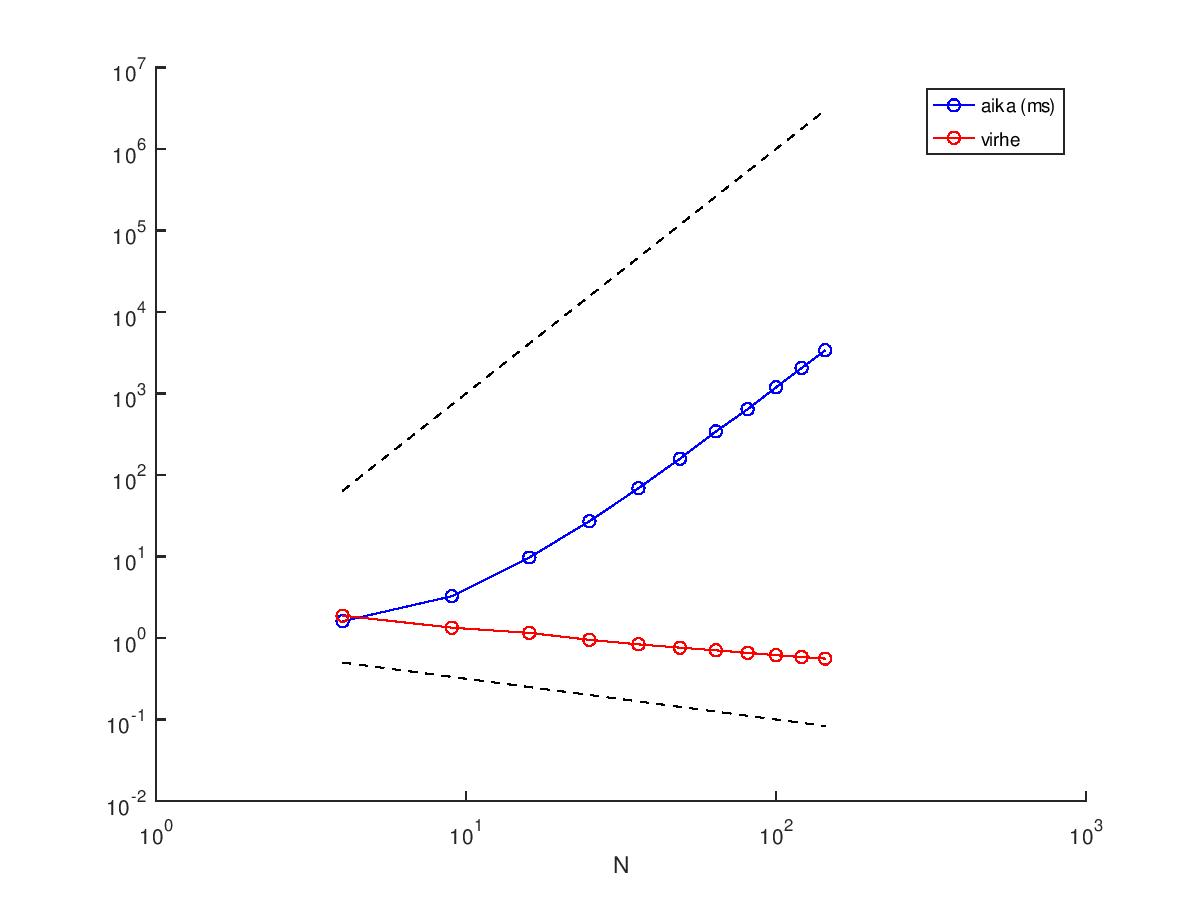
\includegraphics[width=350pt]{w6_2.jpg}

Algoritmin aikavaativuus on kertaluokkaa $O(n^3)$, ja kulunut aika näyttää
vastaavan sitä varsin tar\-kasti.  Virhe puolestaan vaikuttaisi olevan suoraan
verrannollinen hilaväliin, mikä oli differenssi\-menetelmäs\-sä odotettua.

\newpage
\section*{4.-5.}

Valitsin menetelmän tähänkin tehtävään sen perusteella, mikä tuntuu itselleni
hyödyllisimmältä opetella. Jacobi-iteraatio on minulle tähän mennessä tuttu
vain nimeltä, mutta tiedän, että se on hyödyllinen, jos haluan joskus toteuttaa
projekteissani rinnakkaistettua fysiikkaa. Tähän mennessä olen käyttänyt vain
Gauss-Seidel-menetelmiä, joissa järjestys on määrätty. Siksi päätin nyt
tutustua tarkemmin tähän menetelmään. SOR- ja multigrid-metodien aikavaativuus
olisi matalampi, joten todellisuudessa kannattaisi todennäköisesti suosia
niitä.

Käytin tässä uudelleen edellisessä tehtävässä rakennettua matlab-tehtävää
lisäten vain Jacobi-rat\-kaisijan yhtälöryhmälle:

\verbatiminput{w6_jacobi.m}

Lopputulos:

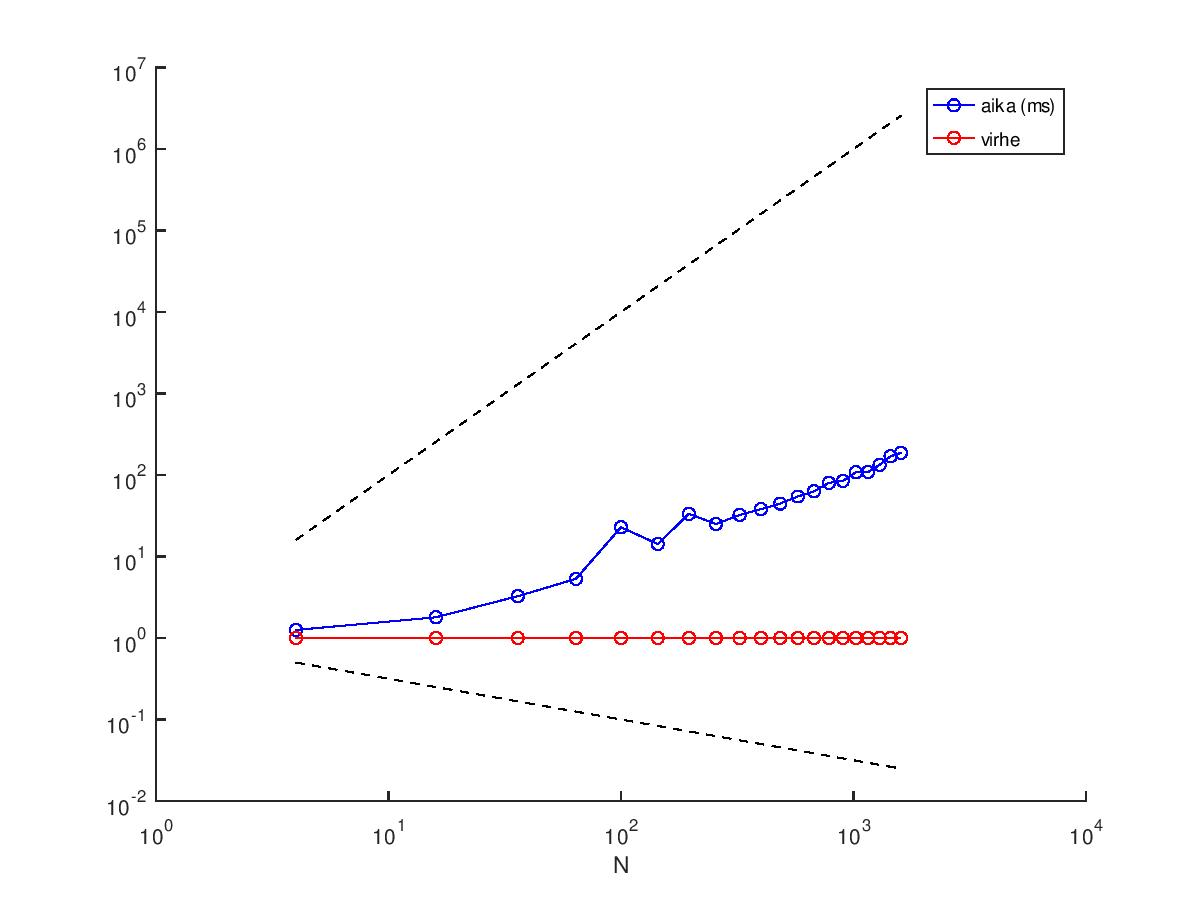
\includegraphics[width=350pt]{w6_4.jpg}

Tässä vertailukohtana ajalle on $y = N^2$, joka vastaa Jacobi-menetelmän
aikavaativuuden kertaluokkaa. Laskenta-aika ei muutu yhtä tasaisesti kuin
edellisen tehtävän käyrä, luultavasti koska matriisin koko ei vaikuta täysin
lineaarisesti konvergenssiin tarvittavaan iteraatiomäärään.  Yllättäen
laskenta-aika näyttää kasvavan hitaammin kuin aikavaativuudesta odottaisi.
Tämä liittyy ehkä matriisin yhteensopivuuteen menetelmän kanssa — arvaan, että
tarvittavien iteraatioiden lukumäärä kasvaa koon suhteen tässä hitaammin kuin
satunnaisella matriisilla. En ehdi nyt tutkia tätä tämän tarkemmin.

Virhe ei muutu, koska käytän konvergenssiehtona virheen laskemista tietyn tason
alapuolelle.

\end{document}
